\documentclass[conference]{IEEEtran}
\usepackage[utf8]{inputenc}
\usepackage[T1]{fontenc}
\usepackage[brazil]{babel}
\usepackage{graphicx}
\usepackage{booktabs}
\usepackage{amsmath}
\usepackage{url}
\usepackage{microtype}
\graphicspath{{figuras/}}

\begin{document}

\title{Detecção de Placas Veiculares com MobileNetV1 e\\
Detector por Grade Embarcado em ESP32-S3}

\author{
\IEEEauthorblockN{Carlos Vinícius dos Santos Mesquita,
Alisson Jaime Sales Barros,\\
Victor Guedes Alves Teixeira e
Kaique Ferreira Braga Silva}
\IEEEauthorblockA{TI0147 --- Fundamentos de Processamento Digital de Imagens\\
Professor: Paulo Cesar Cortez\\
Universidade Federal do Ceará}
}

\maketitle

\begin{abstract}
Este trabalho apresenta um sistema completo de detecção de placas
veiculares baseado na arquitetura MobileNetV1 com uma cabeça de
detector por grade (saída espacial $7\times7\times5$), treinado em
TensorFlow/Keras e embarcado em uma placa ESP32-S3 com câmera OV5640.
O modelo foi quantizado em INT8 e convertido para TensorFlow Lite, viabilizando a
inferência diretamente no microcontrolador. Avaliamos o sistema em três
modalidades (imagem, vídeo e captura em tempo real com a ESP32-CAM), comparamos o
desempenho entre PC e dispositivo embarcado, e aplicamos pós-processamento com
filtragem por confiança e segmentação dos caracteres. Os resultados, obtidos sobre
cinco execuções, mostram IoU médio de $0{,}731\pm0{,}005$ no conjunto
combinado e \emph{recall} de $0{,}922$, com a quantização INT8 preservando a
qualidade (IoU praticamente idêntico ao modelo Keras). A inferência custa
$\sim$4--7~ms no PC contra $\sim$117~s na ESP32-S3, evidenciando o gargalo do
hardware embarcado. O acréscimo de imagens negativas reduziu os falsos positivos a
zero no limiar $0{,}95$.
\end{abstract}

\begin{IEEEkeywords}
detecção de objetos, MobileNetV1, TensorFlow Lite, sistemas embarcados, ESP32,
quantização INT8, processamento digital de imagens.
\end{IEEEkeywords}

\section{Introdução}
A detecção de objetos é uma tarefa central da Visão Computacional, consistindo em
localizar objetos de interesse por meio de \emph{bounding boxes}. Sua execução em
sistemas embarcados, contudo, é desafiadora: dispositivos como a ESP32 possuem
forte restrição de memória e processamento. Arquiteturas da família MobileNet,
baseadas em convoluções separáveis em profundidade (\emph{depthwise separable
convolutions}), foram projetadas para esse cenário, reduzindo parâmetros e custo
computacional.

Este trabalho desenvolve, treina e embarca um detector de placas veiculares
usando MobileNetV1 com uma cabeça de detecção por grade, e o avalia nas três
modalidades exigidas (imagem, vídeo e tempo real). Além do embarcamento na
ESP32-S3, o mesmo modelo é executado em PC para comparação de desempenho, e o
sistema é complementado por pós-processamento (filtragem por confiança e
segmentação dos caracteres da placa).

\section{Base de Dados}
Foram utilizadas duas bases de detecção de objetos de classe única (\texttt{plate}),
com anotações no formato YOLO (centro, largura e altura normalizados):
\textbf{Base~1}, fornecida pelo professor, e \textbf{Base~2}, a base pública
\emph{Brazil Plates Detector} (Roboflow, licença CC~BY~4.0), escolhida pela
aderência ao problema. As bases foram combinadas com ponderação da Base~2 para
reforçar exemplos difíceis. A Tabela~\ref{tab:dados} resume a divisão efetivamente
utilizada. Adicionalmente, incorporamos \textbf{16 imagens negativas} (cenas sem
placa) para reduzir falsos positivos.

\begin{table}[!t]
\centering
\caption{Divisão da base utilizada (uma classe: \texttt{plate}).}
\label{tab:dados}
\begin{tabular}{lcc}
\toprule
Conjunto & Treino & Validação\\
\midrule
Base 1 (professor)        & 350 & 60\\
Base 2 (Brazil Plates)    & 200 & 12\\
Mix ponderado             & 972 & 72\\
Negativas (sem placa)     & 12  & 4\\
\bottomrule
\end{tabular}
\end{table}

\section{Arquitetura e Detector por Grade}
A arquitetura é a \textbf{MobileNetV1} com fator de largura (\emph{width
multiplier}) $\alpha=0{,}5$ e entrada $224\times224\times3$. Sobre o
\emph{backbone} \textbf{pré-treinado na ImageNet} adicionamos uma \textbf{cabeça de detecção por grade}
que produz uma saída espacial $7\times7\times5$: a imagem é dividida em uma grade
$7\times7$ e cada célula prevê uma confiança de objetos (\emph{objectness}) e os
quatro parâmetros da caixa $(c_x, c_y, w, h)$. A detecção final corresponde à
célula de \textbf{maior confiança}, e a caixa global é reconstruída por
$c_x = (\text{col}+c_x^{local})/7$ e $c_y = (\text{lin}+c_y^{local})/7$. Essa
formulação resolveu o problema de localização da região correta da placa observado
em abordagens de regressão direta de uma única caixa. A escolha do MobileNetV1
$\alpha=0{,}5$ equilibra precisão e tamanho, essencial para o embarcamento.

\section{Metodologia}
\subsection{Pré-processamento}
As imagens são redimensionadas para $224\times224$ e normalizadas para o intervalo
$[-1,1]$ por $x_{norm}=x/127{,}5-1$ (Figura~\ref{fig:preproc}). Em PDI é usual
operar apenas sobre a \textbf{luminância} (imagens de um único canal); a
MobileNetV1, porém, exige entrada de três canais. Para contornar essa limitação
da arquitetura escolhida e ainda assim avaliar o comportamento clássico em tons
de cinza, definimos o modo \textbf{gray3}, em que o canal de luminância é
replicado nos três canais de entrada --- ganhando robustez a variações de cor
entre bases e câmeras ---, além do modo \textbf{RGB} convencional. Os dois modos
foram avaliados e permanecem selecionáveis em tempo de execução no
\emph{frontend}. Durante o treino aplicamos \emph{Data Augmentation}:
espelhamento horizontal, variações de brilho/contraste, ruído e desfoque
(Figura~\ref{fig:preproc}e).

\begin{figure*}[!t]
\centering
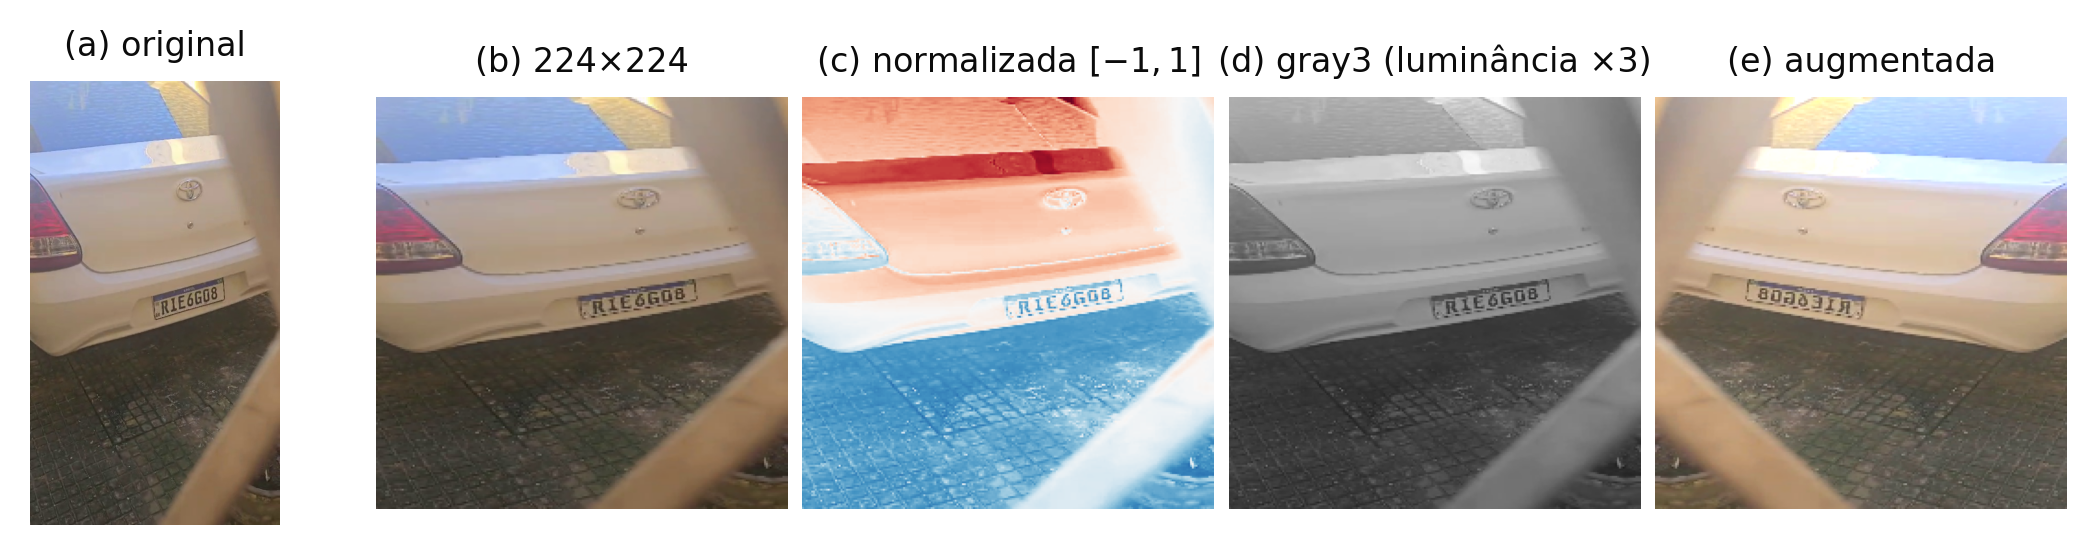
\includegraphics[width=0.96\textwidth]{fig_preproc.png}
\caption{Pré-processamento passo a passo: (a) imagem original; (b)
redimensionamento para $224\times224$; (c) normalização para $[-1,1]$
(visualizada em falsa cor); (d) modo gray3 (luminância replicada em três
canais); (e) exemplo de \emph{Data Augmentation} (espelhamento + brilho).}
\label{fig:preproc}
\end{figure*}

\subsection{Treinamento}
O treino emprega o otimizador Adam em duas fases (\emph{transfer learning} seguido
de \emph{fine-tuning} da cabeça): 12 e 50 épocas, \emph{batch} 8, com
\texttt{ReduceLROnPlateau} e \texttt{EarlyStopping}. A função de perda combina
quatro termos com pesos fixos,
\begin{equation}
\mathcal{L} \;=\; 2\,\mathcal{L}_{\text{conf}}^{\text{obj}}
\;+\; 0{,}25\,\mathcal{L}_{\text{conf}}^{\text{noobj}}
\;+\; 8\,\mathcal{L}_{\text{box}}
\;+\; 3\,\mathcal{L}_{\text{GIoU}},
\label{eq:loss}
\end{equation}
em que $\mathcal{L}_{\text{conf}}^{\text{obj}}$ e
$\mathcal{L}_{\text{conf}}^{\text{noobj}}$ são o erro quadrático da confiança,
médio nas células \emph{com} e \emph{sem} objeto (o peso menor das células
vazias evita que a maioria negativa domine o gradiente);
$\mathcal{L}_{\text{box}}$ é a \emph{Smooth-L1} dos parâmetros locais
$(c_x, c_y, w, h)$ na célula positiva; e $\mathcal{L}_{\text{GIoU}}$ é a perda
GIoU da caixa global reconstruída a partir da grade, que maximiza a
sobreposição real entre predição e anotação. Cada configuração foi executada
\textbf{cinco vezes}, reportando-se média e desvio padrão (Seção~\ref{sec:res}). O
ambiente de treino foi o Google Colab (TensorFlow~2.20.0, Python~3.12, GPU
NVIDIA Tesla~T4).

\subsection{Pós-processamento}
Aplicamos \textbf{filtragem por confiança}: a detecção só é considerada válida
quando a confiança ultrapassa um limiar operacional (projetado em $0{,}95$ e
recalibrável em campo; Seção~\ref{sec:res}) e se mantém por
\textbf{2 \emph{frames} consecutivos}, reduzindo disparos espúrios. Em seguida,
realizamos a \textbf{segmentação dos caracteres} da placa (obrigatória) por
técnicas clássicas de OpenCV, ilustradas etapa a etapa na
Figura~\ref{fig:segetapas}: (i) recorte da ROI prevista; (ii) equalização local
de contraste (CLAHE); (iii) transformação \emph{BlackHat}, que realça
estruturas escuras (caracteres) sobre fundo claro (placa); (iv)
\textbf{limiarização de Otsu} sobre o resultado --- o método escolhe
automaticamente o limiar que maximiza a variância entre as classes
fundo/caractere do histograma (Figura~\ref{fig:segetapas}d) --- combinada com
limiar adaptativo; e (v) limpeza morfológica com filtragem de componentes
conectados por área e proporção. A Figura~\ref{fig:seg} mostra o resultado
sobre um quadro de vídeo e a Figura~\ref{fig:segex} apresenta exemplos
adicionais em fotografias reais capturadas para o trabalho.

\begin{figure}[!t]
\centering
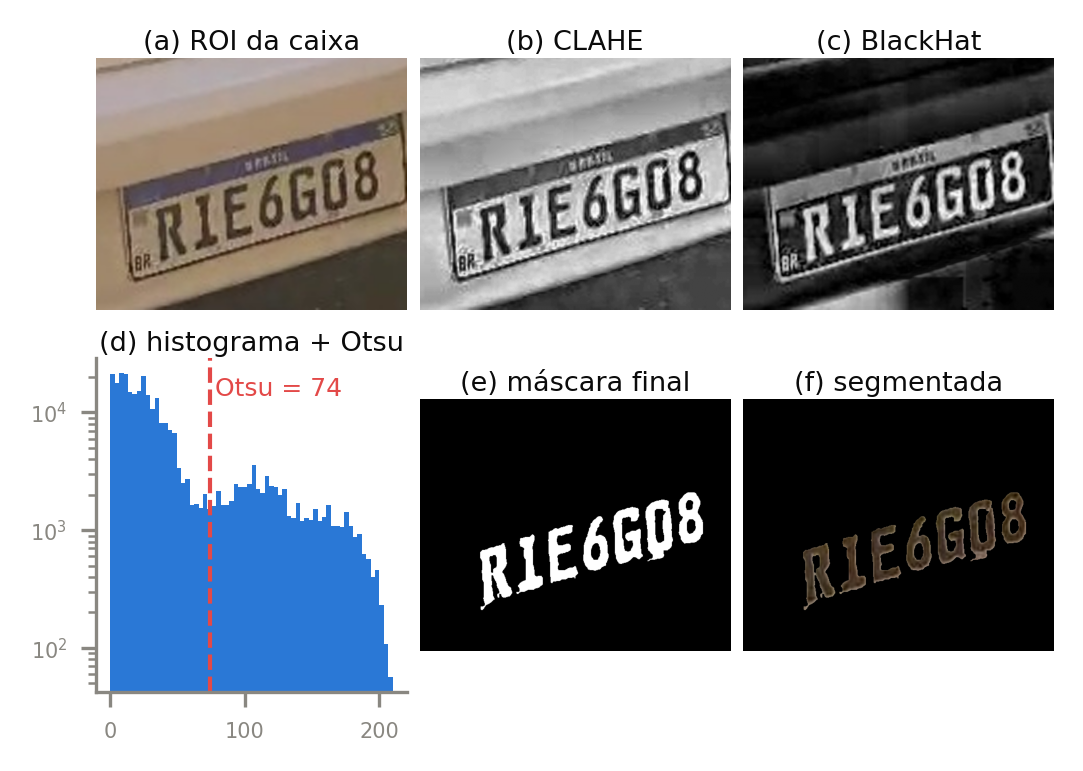
\includegraphics[width=\columnwidth]{fig_seg_etapas.png}
\caption{Etapas da segmentação: (a) ROI recortada da caixa prevista; (b) CLAHE;
(c) BlackHat; (d) histograma do BlackHat com o limiar de Otsu selecionado
(linha tracejada); (e) máscara após limpeza morfológica; (f) caracteres
segmentados.}
\label{fig:segetapas}
\end{figure}

\begin{figure}[!t]
\centering
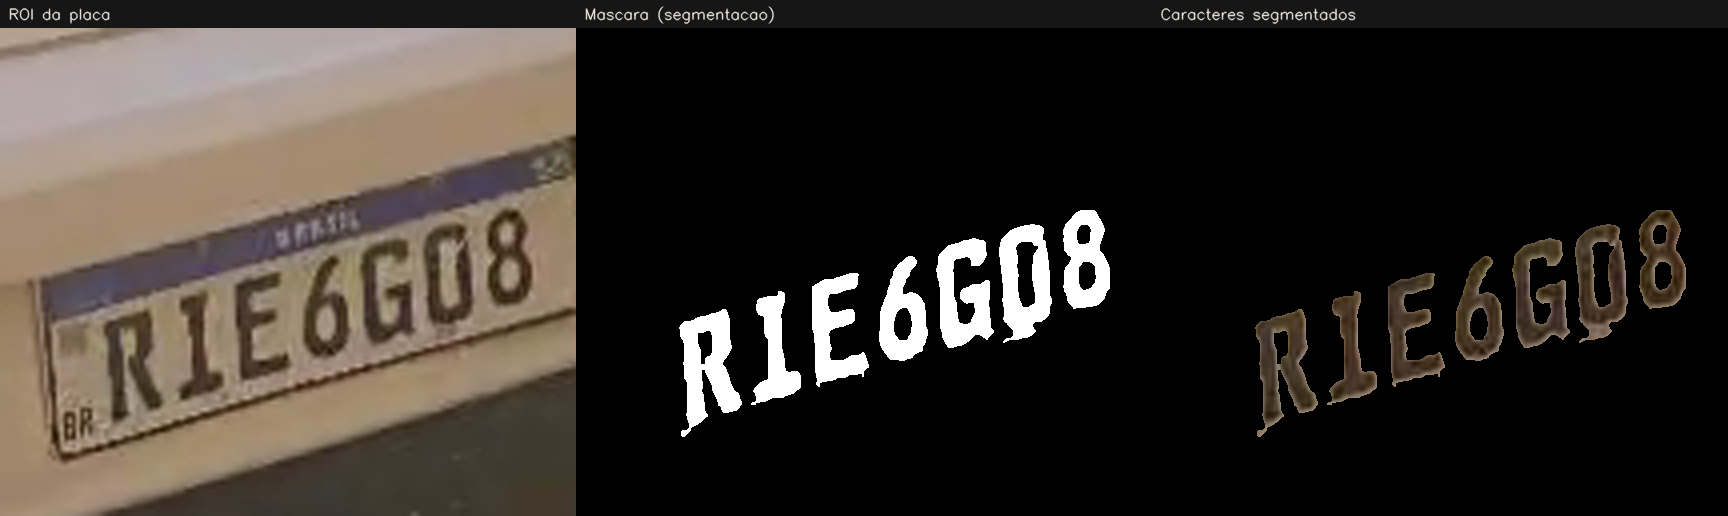
\includegraphics[width=\columnwidth]{fig_segmentacao.png}
\caption{Pós-processamento: ROI da placa, máscara de segmentação e caracteres
segmentados (OpenCV).}
\label{fig:seg}
\end{figure}

\begin{figure}[!t]
\centering
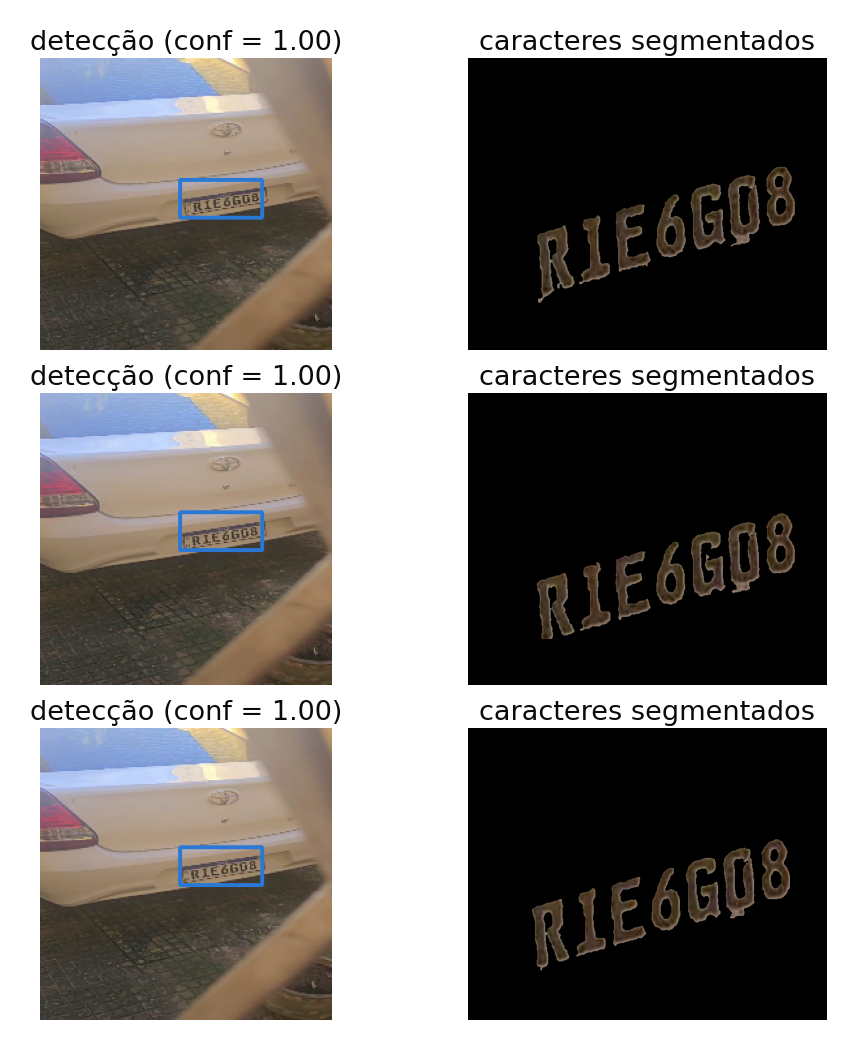
\includegraphics[width=0.92\columnwidth]{fig_seg_exemplos.png}
\caption{Exemplos adicionais de detecção e segmentação em três fotografias
reais (conjunto \texttt{imagens\_teste}).}
\label{fig:segex}
\end{figure}

\subsection{Conversão e Quantização para a ESP32}
O modelo Keras foi convertido para TensorFlow Lite em três variantes (Float32,
\emph{dynamic} e INT8). A quantização \textbf{INT8 pós-treinamento} foi escolhida
para o embarcamento. O arquivo \texttt{.tflite} (2{,}35~MB) foi convertido em um
\emph{array} C++ (\texttt{xxd -i}), gerando um cabeçalho de \textbf{2.468.584
bytes}. No firmware (Arduino/ESP-IDF, biblioteca
\texttt{TensorFlowLite\_ESP32}), o \emph{tensor arena} ($\sim$3{,}4~MB) é alocado
na PSRAM e uma tabela de partições personalizada de 5~MB acomoda o aplicativo
(3{,}74~MB de \emph{flash}). A placa é uma \textbf{ESP32-S3} (16~MB \emph{flash},
8~MB PSRAM OPI, CPU a 240~MHz) com câmera \textbf{OV5640}.

\subsection{Condições Experimentais}
O \textbf{treinamento e a avaliação das métricas} foram realizados no Google Colab
(TensorFlow~2.20.0, Python~3.12, GPU NVIDIA Tesla~T4). Os \textbf{testes em PC}
(execução LiteRT/TFLite) usaram um notebook com CPU Intel Core i7-14700HX, 16~GB de
RAM, Windows~11 (64~bits), Python~3.14. O \textbf{dispositivo embarcado} é uma
ESP32-S3 (16~MB \emph{flash}, 8~MB PSRAM OPI, CPU a 240~MHz) com câmera OV5640,
usando a biblioteca \texttt{TensorFlowLite\_ESP32} (Arduino-ESP32~3.3.8 /
ESP-IDF~5.5).

\section{Resultados}\label{sec:res}
\subsection{Desempenho de detecção (cinco execuções)}
A Tabela~\ref{tab:cinco} apresenta as métricas médias e desvios das cinco execuções.
O modelo atinge \emph{recall} elevado na Base~1 e no conjunto combinado; o
desempenho menor na Base~2 reflete sua maior dificuldade e menor tamanho. O
\emph{score balanceado} indicado na tabela é a média simples dos IoU médios das
duas bases, $(\text{IoU}_{B1}+\text{IoU}_{B2})/2$ --- critério usado para
selecionar o modelo final sem favorecer a base maior.

\begin{table}[!t]
\centering
\caption{Métricas em cinco execuções (média $\pm$ desvio).}
\label{tab:cinco}
\begin{tabular}{lccc}
\toprule
Métrica & Base 1 & Base 2 & Mix\\
\midrule
IoU médio          & $0{,}768\pm0{,}002$ & $0{,}543\pm0{,}030$ & $0{,}731\pm0{,}005$\\
Recall (IoU$\ge$0,5) & $0{,}973\pm0{,}013$ & $0{,}667\pm0{,}075$ & $0{,}922\pm0{,}014$\\
F1@0,5             & $0{,}983$ & $0{,}750$ & $0{,}944$\\
\bottomrule
\end{tabular}
\par\smallskip
\footnotesize Score balanceado (média dos IoU de B1 e B2): $0{,}655\pm0{,}015$.
\end{table}

\subsection{Comparação PC vs.\ ESP32 e validação da quantização}
A Tabela~\ref{tab:plat} compara plataformas e a Figura~\ref{fig:tempolog}
resume os tempos em escala logarítmica. A quantização INT8 \textbf{preservou a
qualidade} (IoU praticamente idêntico ao Keras), reduzindo o modelo de 8{,}75~MB
(Float32) para 2{,}35~MB. No PC a inferência custa poucos milissegundos; na
ESP32-S3, $\sim$117~s por \emph{frame}, cerca de $1{,}7\times10^{4}$ vezes mais
lenta. O gargalo decorre dos \emph{kernels} de referência da biblioteca
TFLite~Micro e do acesso à PSRAM, não do modelo em si.

\begin{figure}[!t]
\centering

\includegraphics[width=0.95\columnwidth]{fig_tempo_log.png}
\caption{Tempo de inferência do mesmo modelo em cada plataforma (escala
logarítmica). O arquivo INT8 é idêntico no PC e na ESP32-S3.}
\label{fig:tempolog}
\end{figure}

\begin{table}[!t]
\centering
\caption{Tempo de inferência, tamanho e IoU (conjunto Mix).}
\label{tab:plat}
\begin{tabular}{lccc}
\toprule
Plataforma / modelo & Tempo & Tamanho & IoU\\
\midrule
Keras (PC, float)        & $\sim$96{,}9~ms & n/d      & 0,736\\
TFLite Float32 (PC)      & $\sim$6{,}5~ms  & 8,75~MB  & 0,736\\
TFLite INT8 (PC, LiteRT) & $\sim$4--7~ms   & 2,35~MB  & 0,732\\
\textbf{TFLite INT8 (ESP32-S3)} & $\sim$\textbf{117~s} & 2,35~MB & n/d\\
\bottomrule
\end{tabular}
\end{table}

\subsection{Efeito das imagens negativas}
A Tabela~\ref{tab:neg} mostra os falsos positivos sobre imagens sem placa em
função do limiar. No limiar adotado ($0{,}95$) não há falsos positivos, e os
exemplos positivos não foram degradados (confiança média $\sim0{,}99$). Medições
na própria ESP32-S3 confirmaram o ganho: cenas sem placa caíram de $\sim0{,}62$
(modelo antigo) para $0{,}42$--$0{,}58$, enquanto uma placa real bem enquadrada
atinge $0{,}98$--$0{,}99$.

\begin{table}[!t]
\centering
\caption{Falsos positivos em imagens sem placa por limiar.}
\label{tab:neg}
\begin{tabular}{lcccc}
\toprule
Limiar & 0,50 & 0,90 & 0,95 & 0,98\\
\midrule
Falsos positivos & 4/4 & 1/4 & \textbf{0/4} & 0/4\\
\bottomrule
\end{tabular}
\end{table}

\subsection{Avaliação nas três modalidades}
\textbf{Imagem.} A Figura~\ref{fig:det} mostra a detecção em uma imagem: a caixa é
posicionada corretamente sobre a placa e o mapa de confiança da grade destaca a
célula correta.

\begin{figure}[!t]
\centering
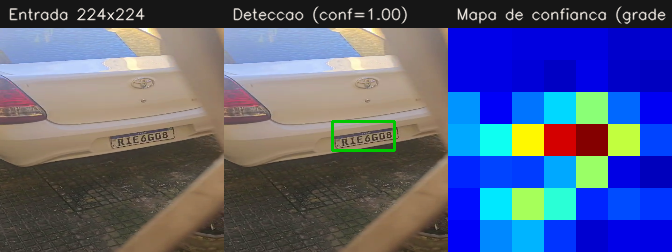
\includegraphics[width=\columnwidth]{fig_deteccao.png}
\caption{Detecção em imagem: entrada, caixa prevista (confiança $\approx1{,}0$) e
mapa de confiança da grade $7\times7$.}
\label{fig:det}
\end{figure}

\textbf{Vídeo.} O modelo foi executado quadro a quadro sobre uma
sequência de vídeo (Figura~\ref{fig:frame}), atingindo confiança de até $0{,}996$
no melhor \emph{frame}, com taxa de processamento de centenas de FPS no PC.

\begin{figure}[!t]
\centering
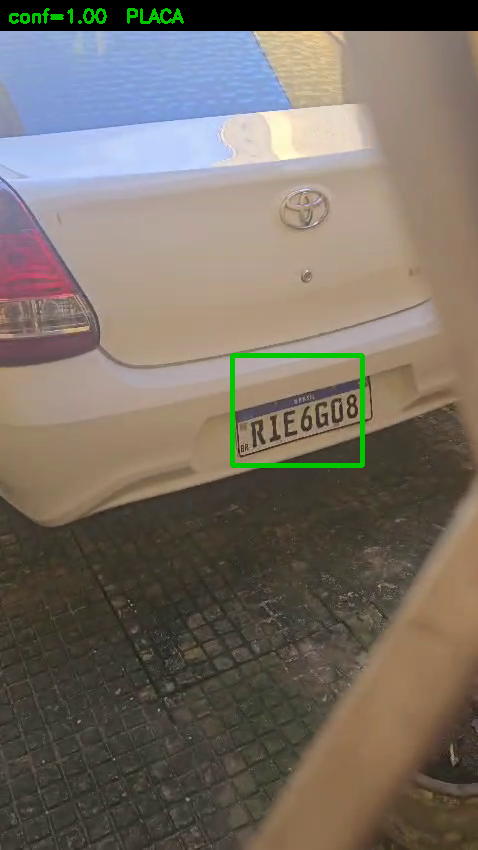
\includegraphics[width=0.62\columnwidth]{fig_frame_anotado.png}
\caption{Detecção em vídeo (melhor \emph{frame}, confiança $0{,}996$).}
\label{fig:frame}
\end{figure}

\textbf{Tempo real.} A captura ao vivo com a OV5640 acoplada à ESP32-S3 produziu
detecção embarcada com confiança $0{,}97$, disparando o envio automático da imagem
anotada (Telegram). A Figura~\ref{fig:semplaca} ilustra a correta \emph{rejeição}
de um quadro sem placa nítida (confiança abaixo do limiar).

A Figura~\ref{fig:campo} registra uma sessão completa de operação em campo
(02/07): cada ponto é uma inferência embarcada ($\sim$117~s). Observa-se que a
confiança com placa presente depende do enquadramento e da iluminação da cena
--- nessa sessão, o platô ficou em $0{,}82$--$0{,}92$, abaixo dos
$0{,}95$--$0{,}99$ obtidos em cenas bem iluminadas. Por isso o limiar de disparo
é tratado como \textbf{parâmetro de operação calibrável em campo} (entre
$0{,}85$ e $0{,}95$, sempre acima da faixa sem placa de $0{,}42$--$0{,}58$): com
o limiar recalibrado para $0{,}85$, dois \emph{frames} consecutivos válidos
dispararam o envio, e a fotografia anotada chegou ao Telegram \textbf{18~s}
após a detecção. A exigência de 2 \emph{frames} consecutivos manteve-se
efetiva: oscilações isoladas abaixo do limiar zeraram a contagem sem gerar
disparos espúrios.

\begin{figure*}[!t]
\centering

\includegraphics[width=0.9\textwidth]{fig_confianca_campo.png}
\caption{Sessão de operação em campo (02/07): confiança por inferência na
ESP32-S3, limiar de disparo recalibrado em campo (linha tracejada), faixa sem
placa medida (área sombreada) e disparo do Telegram após 2 \emph{frames}
consecutivos acima do limiar.}
\label{fig:campo}
\end{figure*}

\begin{figure}[!t]
\centering
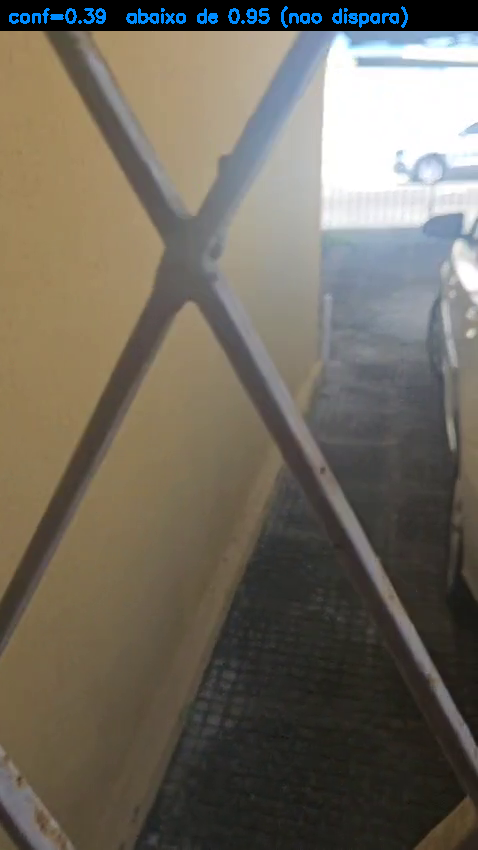
\includegraphics[width=0.62\columnwidth]{fig_sem_placa.png}
\caption{Rejeição correta: quadro sem placa nítida, confiança abaixo do limiar.}
\label{fig:semplaca}
\end{figure}

\section{Discussão}
A quantização INT8 mostrou-se vantajosa: reduziu o modelo em $\sim$73\% sem perda
mensurável de IoU, viabilizando o embarcamento. A principal limitação é o
\textbf{tempo de inferência na ESP32-S3} ($\sim$117~s/\emph{frame}), atribuível aos
\emph{kernels} de referência da TFLite~Micro e à latência da PSRAM, e não ao
tamanho do modelo, já que o mesmo arquivo roda em milissegundos no PC. As imagens
negativas eliminaram os falsos positivos no limiar de operação. A qualidade da
câmera OV5640 e o desfoque por movimento afetam a confiança, mitigados por bom
enquadramento e pela exigência de detecção estável por múltiplos \emph{frames}.

\section{Conclusão e Trabalhos Futuros}
Desenvolvemos um detector de placas com MobileNetV1 e cabeça por grade, embarcado e
funcional na ESP32-S3, avaliado nas três modalidades e comparado ao PC. A solução é
viável e precisa, com a quantização preservando a qualidade. Como trabalhos
futuros: (i) acelerar a inferência embarcada com \emph{kernels} otimizados (ESP-NN)
ou entrada menor ($96\times96$); (ii) alternativamente, transmitir a captura da
ESP32-CAM para inferência em servidor (\emph{frontend} fluido); (iii) ampliar a
base de negativas com fotos capturadas pela própria ESP-CAM; e (iv) reconhecimento
óptico (OCR) dos caracteres já segmentados.

\begin{thebibliography}{9}
\bibitem{mobilenet} A. G. Howard \emph{et al.}, ``MobileNets: Efficient Convolutional
Neural Networks for Mobile Vision Applications,'' arXiv:1704.04861, 2017.
\bibitem{tf} M. Abadi \emph{et al.}, ``TensorFlow: Large-Scale Machine Learning on
Heterogeneous Systems,'' 2015. [Online]. Disponível: \url{https://www.tensorflow.org}
\bibitem{tflite} ``TensorFlow Lite / LiteRT Guide.'' [Online]. Disponível:
\url{https://www.tensorflow.org/lite}
\bibitem{roboflow} Roboflow, ``Brazil Plates Detector Dataset.'' [Online]. Disponível:
\url{https://universe.roboflow.com/testes-bbb7m/brazil-plates-detector-zn2t0}
\bibitem{keras} F. Chollet \emph{et al.}, ``Keras.'' [Online]. Disponível:
\url{https://keras.io}
\bibitem{espidf} Espressif, ``ESP-IDF / ESP32-S3 Technical Reference.'' [Online].
Disponível: \url{https://docs.espressif.com}
\end{thebibliography}

\end{document}
